\documentclass[11pt]{article}
% Shared preamble for the Svetoch papers.
% Each paper.tex \input's this file (compile from inside the paper's folder):
%     \documentclass[11pt]{article}
%     % Shared preamble for the Svetoch papers.
% Each paper.tex \input's this file (compile from inside the paper's folder):
%     \documentclass[11pt]{article}
%     % Shared preamble for the Svetoch papers.
% Each paper.tex \input's this file (compile from inside the paper's folder):
%     \documentclass[11pt]{article}
%     \input{../tex/preamble.tex}
% Figures live in ../figures/*.pdf  (graphicspath set below).
\usepackage[utf8]{inputenc}
\usepackage[T1]{fontenc}
\usepackage{lmodern}
\usepackage[a4paper,margin=1in]{geometry}
\usepackage{amsmath,amssymb}
\usepackage{graphicx}
\graphicspath{{../figures/}}
\usepackage{booktabs}
\usepackage{caption}
\captionsetup{font=small,labelfont=bf}
% --- Minimal, siunitx-free unit support (so papers compile on any TeX install) ---
\usepackage{textcomp}
\newcommand{\SI}[2]{#1\,#2}
\newcommand{\si}[1]{#1}
\newcommand{\hertz}{Hz}
\newcommand{\meter}{m}
\newcommand{\centi}{c}
\newcommand{\milli}{m}
\newcommand{\micro}{\textmu}
\newcommand{\second}{s}
\newcommand{\kelvin}{K}
% ---------------------------------------------------------------------------------
\usepackage[colorlinks=true,linkcolor=blue,citecolor=blue,urlcolor=blue]{hyperref}
\usepackage{xcolor}
\definecolor{accent}{HTML}{6366F1}

% Common author block (add affiliation/ORCID if available before publishing)
\newcommand{\svetochauthor}{Oleg Yuryevich Kirichenko \\[4pt]
  \normalsize Independent researcher \\[2pt]
  \normalsize \href{mailto:urevich55@gmail.com}{urevich55@gmail.com} \quad\textbullet\quad GitHub: \href{https://github.com/infosave2007}{@infosave2007}}

\newcommand{\svetochfooter}{%
  \vspace{1em}\noindent\rule{\linewidth}{0.4pt}\\[2pt]
  {\footnotesize Part of the \emph{Svetoch} series (defensive publication, not patented).
  Project and code: \href{https://github.com/infosave2007/svetoch}{github.com/infosave2007/svetoch};
  related VMF/NVG theory: \href{https://github.com/infosave2007/vmf}{github.com/infosave2007/vmf}.
  Released for the public record to establish authorship and priority.}}

% Figures live in ../figures/*.pdf  (graphicspath set below).
\usepackage[utf8]{inputenc}
\usepackage[T1]{fontenc}
\usepackage{lmodern}
\usepackage[a4paper,margin=1in]{geometry}
\usepackage{amsmath,amssymb}
\usepackage{graphicx}
\graphicspath{{../figures/}}
\usepackage{booktabs}
\usepackage{caption}
\captionsetup{font=small,labelfont=bf}
% --- Minimal, siunitx-free unit support (so papers compile on any TeX install) ---
\usepackage{textcomp}
\newcommand{\SI}[2]{#1\,#2}
\newcommand{\si}[1]{#1}
\newcommand{\hertz}{Hz}
\newcommand{\meter}{m}
\newcommand{\centi}{c}
\newcommand{\milli}{m}
\newcommand{\micro}{\textmu}
\newcommand{\second}{s}
\newcommand{\kelvin}{K}
% ---------------------------------------------------------------------------------
\usepackage[colorlinks=true,linkcolor=blue,citecolor=blue,urlcolor=blue]{hyperref}
\usepackage{xcolor}
\definecolor{accent}{HTML}{6366F1}

% Common author block (add affiliation/ORCID if available before publishing)
\newcommand{\svetochauthor}{Oleg Yuryevich Kirichenko \\[4pt]
  \normalsize Independent researcher \\[2pt]
  \normalsize \href{mailto:urevich55@gmail.com}{urevich55@gmail.com} \quad\textbullet\quad GitHub: \href{https://github.com/infosave2007}{@infosave2007}}

\newcommand{\svetochfooter}{%
  \vspace{1em}\noindent\rule{\linewidth}{0.4pt}\\[2pt]
  {\footnotesize Part of the \emph{Svetoch} series (defensive publication, not patented).
  Project and code: \href{https://github.com/infosave2007/svetoch}{github.com/infosave2007/svetoch};
  related VMF/NVG theory: \href{https://github.com/infosave2007/vmf}{github.com/infosave2007/vmf}.
  Released for the public record to establish authorship and priority.}}

% Figures live in ../figures/*.pdf  (graphicspath set below).
\usepackage[utf8]{inputenc}
\usepackage[T1]{fontenc}
\usepackage{lmodern}
\usepackage[a4paper,margin=1in]{geometry}
\usepackage{amsmath,amssymb}
\usepackage{graphicx}
\graphicspath{{../figures/}}
\usepackage{booktabs}
\usepackage{caption}
\captionsetup{font=small,labelfont=bf}
% --- Minimal, siunitx-free unit support (so papers compile on any TeX install) ---
\usepackage{textcomp}
\newcommand{\SI}[2]{#1\,#2}
\newcommand{\si}[1]{#1}
\newcommand{\hertz}{Hz}
\newcommand{\meter}{m}
\newcommand{\centi}{c}
\newcommand{\milli}{m}
\newcommand{\micro}{\textmu}
\newcommand{\second}{s}
\newcommand{\kelvin}{K}
% ---------------------------------------------------------------------------------
\usepackage[colorlinks=true,linkcolor=blue,citecolor=blue,urlcolor=blue]{hyperref}
\usepackage{xcolor}
\definecolor{accent}{HTML}{6366F1}

% Common author block (add affiliation/ORCID if available before publishing)
\newcommand{\svetochauthor}{Oleg Yuryevich Kirichenko \\[4pt]
  \normalsize Independent researcher \\[2pt]
  \normalsize \href{mailto:urevich55@gmail.com}{urevich55@gmail.com} \quad\textbullet\quad GitHub: \href{https://github.com/infosave2007}{@infosave2007}}

\newcommand{\svetochfooter}{%
  \vspace{1em}\noindent\rule{\linewidth}{0.4pt}\\[2pt]
  {\footnotesize Part of the \emph{Svetoch} series (defensive publication, not patented).
  Project and code: \href{https://github.com/infosave2007/svetoch}{github.com/infosave2007/svetoch};
  related VMF/NVG theory: \href{https://github.com/infosave2007/vmf}{github.com/infosave2007/vmf}.
  Released for the public record to establish authorship and priority.}}


\title{\textbf{A Thermo-Optical Convection Layer above an OLED Display\\
as a Programmable Analog Medium}\\[4pt]
{\large Svetoch Series, Paper III of V}}
\author{\svetochauthor}
\date{17 June 2026 \quad\textbullet\quad preprint / defensive publication (not patented)}

\begin{document}
\maketitle

\begin{abstract}
\noindent The companion papers in this series route light from a smartphone's OLED screen to
its front camera with an external flat mirror. Here we remove the mirror and ask whether the
\emph{air itself} can close the loop. With the phone lying screen-up, the heated OLED warms a
thin layer of air above the cover glass; buoyancy drives a laminar natural-convection boundary
layer whose temperature --- and hence refractive-index --- field is set, pixel by pixel, by
what the screen displays. The air becomes an unmodified, programmable phase spatial light
modulator (SLM), written by the OLED and read by the front camera through Background-Oriented
Schlieren (BOS). From first principles, a Rayleigh number $Ra\approx 6.2\times10^{6}$
(laminar, $Ra<10^{9}$) yields a thermal-layer thickness $\delta_T\approx L\,Ra^{-1/5}\approx
6.9$\,mm matching the screen-to-camera gap; the Edl\'en relation $\mathrm{d}n/\mathrm{d}T\approx
-9.4\times10^{-7}\,\mathrm{K^{-1}}$ turns a $\Delta T=20\,^{\circ}\mathrm{C}$ heating into
$\Delta n\approx -1.8\times10^{-5}$; a $\Lambda=4$\,mm thermal grating deflects rays by
$\theta_x\approx -6.6\times10^{-5}$\,rad ($\sim0.41$\,px, sub-pixel, BOS-recoverable); and the
optical-path difference (OPD $\approx126$\,nm) gives a $\sim85^{\circ}$ phase shift and visible
Fabry--P\'erot moir\'e. The demonstrated effect is a \textbf{low-SNR ($\approx1.3$) sub-pixel
deflection}, with controlled shifts up to $\sim1.6$--$2.0$ equivalent pixels under $\times15$
upscaling. We outline applications --- resonant aerosol actuation, mobile schlieren/leak
imaging, and a speculative ``air-as-coprocessor'' matrix engine --- and state plainly which are
demonstrated and which remain conjectural pending higher SNR.
\end{abstract}

\noindent\textbf{Keywords:} Background-Oriented Schlieren, natural convection, Rayleigh number,
refractive index, Edl\'en equation, phase SLM, OLED, thermo-optics, smartphone sensing, analog
computing.

\section{Introduction}
Paper~I showed that an OLED screen, an inexpensive flat mirror, and a front camera form a self-contained
analog matrix engine. The mirror is the one component not already in the phone. This paper asks
whether it can be eliminated by letting a physical field in the air --- rather than a reflective
surface --- carry the optical signal back to the camera.

A phone lying screen-up is a warm horizontal plate. Driving the OLED bright raises the cover
glass a few degrees above ambient; the air above is heated and rises by buoyancy, forming a
natural-convection thermal boundary layer. Since the refractive index of air depends weakly but
measurably on temperature, the displayed brightness pattern is \emph{written} into the air as a
refractive-index pattern. Light skimming through the layer is deflected, and the front camera
reads the deflection. Waste heat becomes the medium itself.

This is the \textbf{mirror-less channel}: screen $\to$ heated air boundary layer $\to$ camera,
with no added optics (Figure~\ref{fig:device}). The air acts as a programmable phase SLM; the
read-out is Background-Oriented Schlieren (BOS), in which a structured reference background,
distorted by index gradients, is recovered by image cross-correlation --- and here the
reference background is painted by the screen itself.

We state the scientific status at the outset. The original derivation was \emph{inspired by} a
structural analogy to a speculative ``Vacuum Mass Fraction / Null-Vector Gravity'' (VMF/NVG)
picture of the QCD vacuum, mapping a condensate amplitude and Goldstone phase onto the
temperature and flow-potential fields. We treat that analogy strictly as mathematical
scaffolding and engineering inspiration, and make \emph{no} claim about real vacuum or QCD
physics. The actual basis is uncontroversial physics: Navier--Stokes natural convection, the
Rayleigh number, the Edl\'en index relation, schlieren/BOS ray optics, and Fabry--P\'erot
interference.

\begin{figure}[ht]\centering
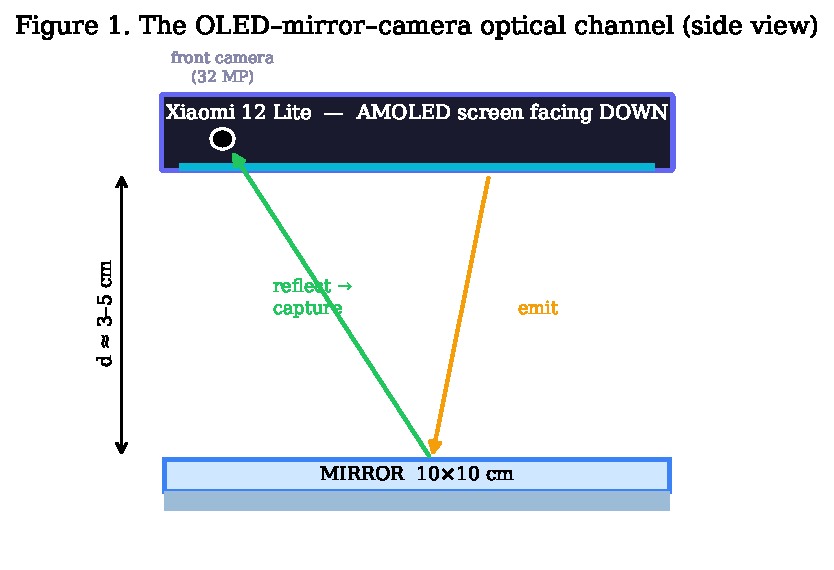
\includegraphics[width=0.74\linewidth]{fig01_device_schematic.pdf}
\caption{Device geometry. For the mirror-less channel the phone lies screen-up; the heated OLED
warms the air boundary layer above the cover glass, which the front camera reads through the
same few-millimetre gap.}
\label{fig:device}
\end{figure}

\section{Theory of the thermal boundary layer}
\subsection{Convection regime and layer thickness}
For a heated horizontal plate the regime is set by the Rayleigh number
\begin{equation}
Ra = \frac{g\,\beta\,\Delta T\, L^{3}}{\nu\,\alpha},
\end{equation}
with $g=9.81\,\mathrm{m\,s^{-2}}$, $\beta=1/T_0\approx 3.3\times10^{-3}\,\mathrm{K^{-1}}$,
$\nu\approx 1.6\times10^{-5}\,\mathrm{m^2\,s^{-1}}$, $\alpha\approx 2.2\times10^{-5}\,
\mathrm{m^2\,s^{-1}}$, $L\approx 0.15$\,m (a 6.55$''$ display), and a full-white heating
$\Delta T=20\,^{\circ}\mathrm{C}$. Then
\begin{equation}
Ra \approx \frac{9.81 \times 3.3\times10^{-3} \times 20 \times 0.15^{3}}
{1.6\times10^{-5}\times 2.2\times10^{-5}} \approx 6.2\times10^{6}.
\end{equation}
Since $Ra<10^{9}$, the flow is firmly \textbf{laminar}, forming a stable convection layer. From
boundary-layer similarity,
\begin{equation}
\delta_T \approx L\,Ra^{-1/5} \approx 0.15\times(6.2\times10^{6})^{-0.2} \approx 6.9\;\mathrm{mm},
\end{equation}
which matches the optical path from the OLED to the front-camera pupil through the cover glass,
$d_\mathrm{gap}\approx 5$--$7$\,mm: the camera light traverses essentially the full depth of the
programmable layer (Figure~\ref{fig:boundary}).

\begin{figure}[ht]\centering
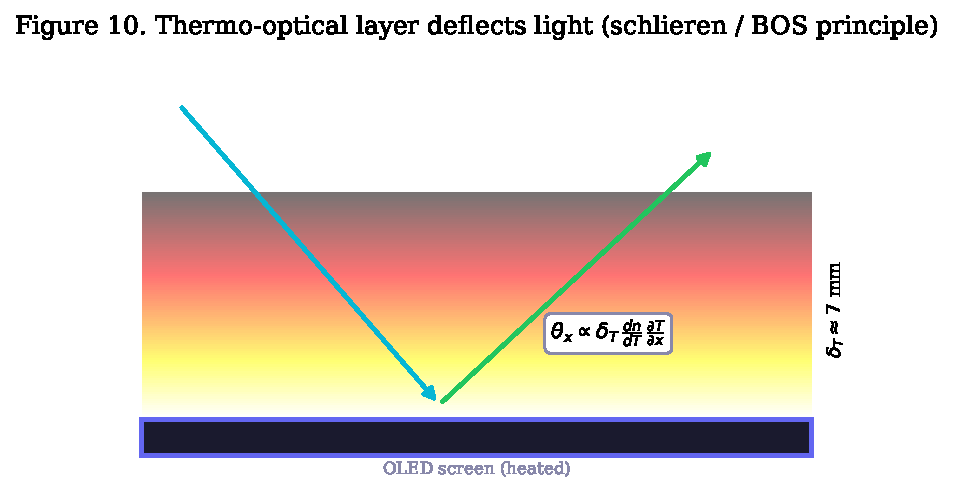
\includegraphics[width=0.8\linewidth]{fig10_thermal_boundary.pdf}
\caption{The thermo-optical layer. Buoyancy above the heated OLED forms a laminar boundary layer
of thickness $\delta_T\approx 7$\,mm; rays crossing its lateral index gradient are deflected by
$\theta_x\approx \delta_T\,(\mathrm{d}n/\mathrm{d}T)\,(\partial T/\partial x)$ and read as a
sub-pixel shift (BOS).}
\label{fig:boundary}
\end{figure}

\subsection{Refractive-index modulation (Edl\'en)}
The temperature dependence of the index of air (Edl\'en, visible, standard pressure) is
\begin{equation}
\frac{\mathrm{d}n}{\mathrm{d}T} \approx -9.4\times10^{-7}\;\mathrm{K^{-1}},
\end{equation}
so a $\Delta T=20\,^{\circ}\mathrm{C}$ contrast writes an index contrast
\begin{equation}
\Delta n = \frac{\mathrm{d}n}{\mathrm{d}T}\,\Delta T \approx -1.8\times10^{-5}.
\end{equation}
Small in absolute terms, but enough for a recoverable signal because both deflection and phase
accumulate over the millimetre-scale layer.

\subsection{Schlieren ray deflection}
A ray crossing a lateral index gradient over the layer depth is deflected by
\begin{equation}
\theta_x = \int_0^{\delta_T}\frac{1}{n}\frac{\partial n}{\partial x}\,\mathrm{d}z
\approx \delta_T\,\frac{\mathrm{d}n}{\mathrm{d}T}\,\frac{\partial T}{\partial x}.
\end{equation}
For a displayed thermal grating of period $\Lambda\approx 4$\,mm (Figure~\ref{fig:profile}), the
edge gradient is
\begin{equation}
\frac{\partial T}{\partial x}\approx \frac{\Delta T}{\Lambda/2}
\approx \frac{20\;\mathrm{K}}{2\times10^{-3}\;\mathrm{m}}\approx 10^{4}\;\mathrm{K\,m^{-1}},
\end{equation}
giving
\begin{equation}
\theta_x \approx (7\times10^{-3}\,\mathrm{m})(-9.4\times10^{-7}\,\mathrm{K^{-1}})
(10^{4}\,\mathrm{K\,m^{-1}}) \approx -6.6\times10^{-5}\;\mathrm{rad}.
\end{equation}
Over the gap this displaces the imaged background by
\begin{equation}
\Delta x_\mathrm{sensor} = d_\mathrm{gap}\,\theta_x \approx
5\times10^{-3}\,\mathrm{m}\times 6.6\times10^{-5}\,\mathrm{rad}\approx 0.33\;\mu\mathrm{m},
\end{equation}
which, at the $0.8\,\mu\mathrm{m}$ front-camera pitch, is
\begin{equation}
\Delta x_\mathrm{px}\approx \frac{0.33\;\mu\mathrm{m}}{0.8\;\mu\mathrm{m/px}}\approx 0.41\;\text{px}.
\end{equation}
A $\sim0.4$\,px shift is sub-pixel but well within BOS cross-correlation, which routinely
resolves $\sim0.05$\,px.

\begin{figure}[ht]\centering
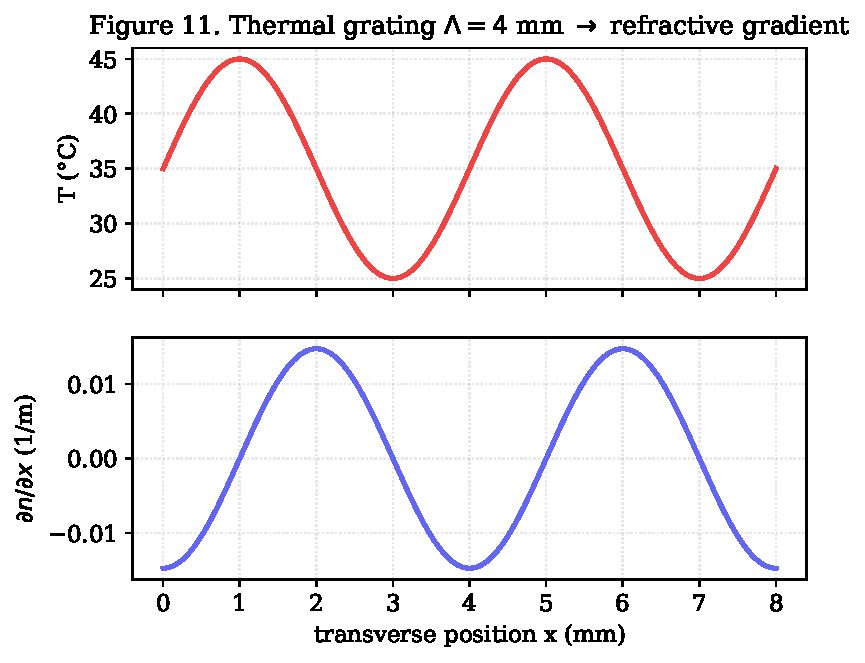
\includegraphics[width=0.7\linewidth]{fig11_refractive_profile.pdf}
\caption{A $\Lambda=4$\,mm thermal grating on the OLED. The temperature profile $T(x)$ and the
resulting lateral index gradient $\partial n/\partial x$ define the deflection field read by the
camera.}
\label{fig:profile}
\end{figure}

\subsection{Fabry--P\'erot moir\'e: the layer as a phase SLM}
The index contrast also accumulates phase along the depth. The optical-path difference between a
hot and a cold column is
\begin{equation}
\mathrm{OPD} = |\Delta n|\,\delta_T \approx 1.8\times10^{-5}\times7\times10^{-3}\,\mathrm{m}
\approx 126\;\mathrm{nm}.
\end{equation}
For the green OLED sub-pixel, $\lambda=532$\,nm, this is
\begin{equation}
\varphi = 2\pi\,\frac{\mathrm{OPD}}{\lambda} = 2\pi\,\frac{126}{532}
\approx 1.49\;\mathrm{rad}\approx 85^{\circ}.
\end{equation}
An $85^{\circ}$ phase shift is large; modulating the multiple-beam Fabry--P\'erot interference
in the cover glass, it produces strong spatial bands --- the moir\'e visible above the glass.
Hence the central claim: the thermal layer is a \textbf{programmable phase spatial light
modulator}, its phase map set by displayed brightness. The screen writes phase into the air;
the camera reads it.

\section{Read-out by Background-Oriented Schlieren}
BOS reconstructs an index-gradient field by comparing a reference frame and a perturbed frame
through local cross-correlation (or block matching, e.g.\ sum-of-absolute-differences) of a
structured background. The pixel displacement $\Delta x(x,y)$ is proportional to the
line-integrated index gradient --- exactly the $\theta_x$ above.

The mirror-less channel supplies its own background: the OLED paints a high-frequency reference
(grating or speckle), captures a cold baseline frame, then heats and captures the perturbed
frame. No external grid, collimator, or knife-edge is needed --- the structured background and
the heat source are the same device.

\paragraph{Measured performance.} The experiment recorded controlled displacements up to
$\sim1.6$--$2.0$ \emph{equivalent} pixels, where the equivalence includes $\times15$ digital
upscaling ($\sim0.1$--$0.13$ physical pixels), consistent with the $\sim0.4$\,px first-principles
estimate to within the model's crudeness. The recovered shift had $\mathrm{SNR}\approx 1.3$:
real but \textbf{weak}, sitting close to the floor set by shot noise, focus breathing, ambient
air currents, and device drift. SNR is the governing figure of merit for every application
below, and raising it is the single most important open problem.

\section{Applications}
\subsection{Resonant thermo-optical actuation of aerosols (strong)}
Displaying a large quad-vortex pattern and modulating its intensity at the convection resonance
($\approx5$\,Hz) drives a macroscopic thermal column. With smoke or aerosol present, the
resonantly amplified flow entrains particles into a visible macro-vortex, which the same camera
quantifies by optical flow. Being a large, directly imaged motion rather than a sub-pixel
deflection, this is the most robustly demonstrated application and the least dependent on BOS SNR.

\subsection{Mobile schlieren / BOS visualizer (strong)}
Section~3 is itself an instrument: a pocket schlieren/BOS visualizer using the screen's own
reference pattern. It images thermal plumes, convection, and gas leaks by detecting index
disturbances above a $3\sigma$ threshold and classifying them by spectral-temporal signature.
The novelty is using the device's own display as the structured BOS background, removing the
bench optics schlieren normally requires.

\subsection{``Air as coprocessor'': thermo-optical matrix multiply (speculative)}
If weights are encoded as a displayed brightness pattern, the induced index gradients implement
a spatial multiply and the BOS-measured deflection integrates a vector--matrix product; eight
heated zones could act as a parallel bus, and vortex chirality could encode an activation sign.
This ``Thermal LLM'' is attractive but \textbf{gated by SNR}: at $\mathrm{SNR}\approx1.3$ per
zone the arithmetic accuracy is far below a useful accelerator's. It is \emph{promising but
speculative pending substantially higher SNR} (e.g.\ acousto-optic high-frequency thermal
modulation, sharper $\partial n/\partial x$ from fine checkerboard masks, or graphene-assisted
heat localization).

\subsection{Further directions (speculative)}
Three further concepts follow from the same physics, reported as conjectures: (B4) computing
\textbf{topological invariants} (Gauss linking numbers) from the optical-flow field of
interacting thermal vortices, with hysteresis as medium memory; (B7) a \textbf{volumetric
aerosol display}, rendering density structures visible in scattered light, with a dry control
frame separating real structure from artifacts; and (B8) a \textbf{contactless thermo-optical
router}, switching a thermal lens/vortex between channels by addressing heated zones. Each is
novel in modality but has uncertain enablement at present SNR.

\section{Methods}
\textbf{Hardware:} Xiaomi 12 Lite (6.55$''$ AMOLED, $2400\times1080$, \SI{120}{\hertz}, OLED
pitch \SI{63.2}{\micro\meter}; 32\,MP front camera, photosite pitch
$\approx$\SI{0.8}{\micro\meter}, min.\ focus $\approx$\SI{10}{\centi\meter}). For the
mirror-less channel the phone lies \emph{screen-up} on a rigid stand in still air; the path is
screen $\to$ cover glass $\to$ heated air layer $\to$ front-camera pupil, gap
$d_\mathrm{gap}\approx 5$--$7$\,mm. \textbf{Protocol:} (1) display a high-frequency reference
($\Lambda\approx 4$\,mm grating, or speckle) and capture a cold baseline; (2) drive the
heating/grating pattern, letting the layer develop over $\tau_\mathrm{thermal}\approx
100$--200\,ms; (3) capture the perturbed frame; (4) recover the displacement by BOS
cross-correlation (block matching, $\times15$ upscaling) and report shift and SNR. For
actuation, modulate a quad-vortex at $\approx5$\,Hz and quantify entrained flow by optical
flow. \textbf{Software:} as in Paper~I, a dependency-free Python HTTPS server relays Start/Stop
and stores runs as JSON; browser ES modules render patterns, capture frames via
\texttt{getUserMedia}, compute the BOS metric, and post results. \textbf{Figures:} theory
figures plot the closed-form relations of Section~2; produced by
\texttt{papers/scripts/make\_figures.py}.

\section{Discussion and limitations}
\textbf{The effect is real but weak.} What is demonstrated is a controlled, repeatable,
sub-pixel deflection produced by displayed heat and recovered by BOS, $\mathrm{SNR}\approx1.3$
--- enough to \emph{visualize} index gradients (4.1--4.2) but not yet to \emph{compute}
reliably (4.3--4.4). The matrix-multiply, router, and volumetric-display applications are
engineering conjectures whose enablement hinges on raising SNR by one to two orders of
magnitude.

\textbf{Patentability framing.} Our internal review rates the actuation (A1) and the mobile
schlieren/BOS visualizer (A6) as strong --- demonstrable effects with narrow claims --- while
the thermal matrix multiply (B5), volumetric display (B7), and router (B8) are moderate, with
enablement risk driven by the low SNR.

\textbf{The VMF/NVG analogy is an analogy.} The condensate-amplitude $\leftrightarrow$
temperature and Goldstone-phase $\leftrightarrow$ flow-potential correspondence is a structural
mnemonic only. Nothing here tests, supports, or depends on any claim about the QCD vacuum; the
physics used stands on its own established footing.

\textbf{Other limitations.} The thermal time constant ($\sim$100--200\,ms) caps the native
modulation rate; ambient currents, focus breathing, and device drift degrade SNR; and the close
$\delta_T\approx d_\mathrm{gap}$ coincidence is device-specific and should be re-derived per phone.

\section{Conclusion}
Removing the mirror, the air above a heated OLED becomes a programmable phase SLM: the screen
writes an index pattern into a laminar convection layer ($Ra\approx6.2\times10^{6}$,
$\delta_T\approx6.9$\,mm), the front camera reads the sub-pixel deflection
($\theta_x\approx-6.6\times10^{-5}$\,rad) by BOS, and a $\sim85^{\circ}$ Fabry--P\'erot phase
shift makes it visible as moir\'e. The channel is genuine but low-SNR ($\approx1.3$); it
already enables resonant aerosol actuation and mobile schlieren imaging, while the compute,
router, and display applications remain promising conjectures pending higher SNR.

\paragraph{Data and code.} \href{https://github.com/infosave2007/svetoch}{github.com/infosave2007/svetoch}; related VMF/NVG theory: \href{https://github.com/infosave2007/vmf}{github.com/infosave2007/vmf}
(Apache-2.0).
\paragraph{Priority note.} Released as a defensive publication to establish authorship and date
of disclosure; the author has elected not to seek patent protection.

\begin{thebibliography}{9}\small
\bibitem{edlen} B. Edl\'en, ``The refractive index of air,'' \emph{Metrologia} \textbf{2}, 71 (1966).
\bibitem{settles} G. S. Settles, \emph{Schlieren and Shadowgraph Techniques}, Springer, 2001.
\bibitem{raffel} M. Raffel, ``Background-oriented schlieren (BOS) techniques,'' \emph{Exp. Fluids} \textbf{56}, 60 (2015).
\bibitem{chandra} S. Chandrasekhar, \emph{Hydrodynamic and Hydromagnetic Stability}, Oxford Univ.\ Press, 1961.
\bibitem{korpel} A. Korpel, \emph{Acousto-Optics}, 2nd ed., Marcel Dekker, 1997.
\bibitem{wetzstein} G. Wetzstein et al., ``Inference in AI with deep optics and photonics,'' \emph{Nature} \textbf{588}, 39 (2020).
\end{thebibliography}

\svetochfooter
\end{document}
